\documentclass[12pt]{article}
\usepackage{a4wide}
\usepackage{latexsym}
\usepackage{amssymb}
\usepackage{amsmath}
\usepackage{amsthm}
\usepackage{commath}
\usepackage{listings}
\usepackage{epic}
\usepackage{graphicx}
\usepackage{float}
\usepackage{hyperref}
\usepackage{algorithm,algorithmic}
%\pagestyle{empty}
\newcommand{\tr}{\mbox{\sf true}}
\newcommand{\fa}{\mbox{\sf false}}
\usepackage[toc,page]{appendix}
\newcommand{\bimp}{\leftrightarrow}
\usepackage{enumitem}
% \renewcommand{\algorithmicrequire}{\textbf{Input:}}
% \renewcommand{\algorithmicensure}{\textbf{Output:}}

\newtheorem{theorem}{Theorem}[section]
\newtheorem{lemma}[theorem]{Lemma}


\usepackage{changepage}
\newcommand\sdent{\begin{adjustwidth}{2.5em}{0pt}}
\newcommand\edent{\end{adjustwidth}}

\begin{document}

\lstset{
    frame=tb,
    aboveskip=3mm,
    belowskip=3mm,
    showstringspaces=false,
    columns=flexible,
    basicstyle={\small\ttfamily},
    numbers=left,                    % where to put the line-numbers; possible values are (none, left, right)
  numbersep=5pt,                   % how far the line-numbers are from the code
  numberstyle=\footnotesize,
  postbreak=\mbox{$\hookrightarrow$\space},
    breaklines=true,
    breakatwhitespace=false,
    tabsize=3,
    frame=shadowbox,
}

\begin{center}
\font\myfont=cmr12 at 30pt
\title*{\myfont Polygon intersection algorithm}
\end{center}

\begin{center}
Tar van Krieken
\end{center}

\vspace{8mm}

\section*{Introduction}
This document describes an algorithm I came up with while following the Geometric Algorithms course (2IMA15) at the Technical University of Eindhoven.

The algorithm calculates the faces that are formed adding multiple simple polygons to the same plane. An example of what separated faces are formed and calculated by the algorithm can be seen in Figure \ref{fig:intersectionExample}

\begin{figure}[!htb]
  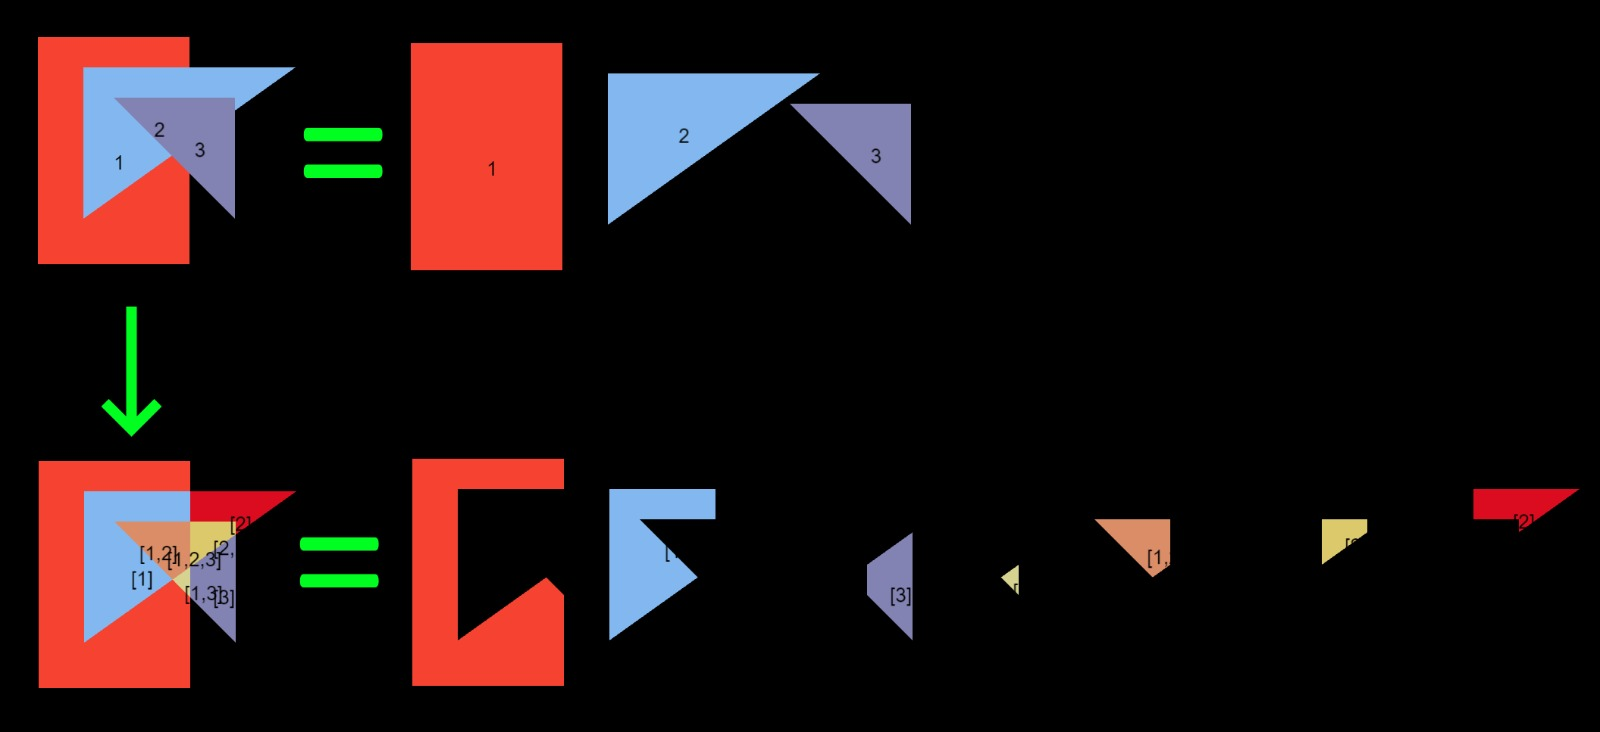
\includegraphics[width=\linewidth]{Images/intersectionExample.jpg}
  \caption{Face separation example}
  \label{fig:intersectionExample}
\end{figure}

The algorithm unfortunately suffers from some robustness issues. An attempt was made to resolve these but without success. A redesign is probably required to fix these issues instead of only applying patches within the implementation. 

\newpage
\section*{Approach}

The algorithm is based on a vertical \href{https://en.wikipedia.org/wiki/Sweep_line_algorithm}{line sweep}. The scanline tracks all separate x-intervals formed by segments that intersect the scanline as illustrated in Figure \ref{fig:intersectionScanline}. The intervals hold the following information:
\begin{itemize}
    \item The left boundary (if any)
    \item The right boundary (if any)
    \item The output shape
\end{itemize}
\begin{figure}[!htb]
  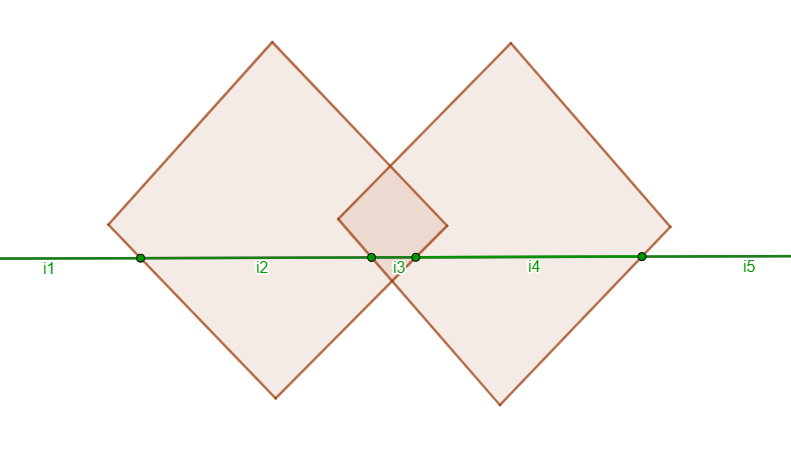
\includegraphics[width=\linewidth]{Images/intersection_scanline.png}
  \caption{The scanline and the intervals it stores}
  \label{fig:intersectionScanline}
\end{figure}

These output shapes are y-monotone polygon sections. Each section contains the following data:
\begin{itemize}
    \item The left walls (A list of points sorted in increasing y-value)
    \item The right walls (A list of points sorted in increasing y-value)
    \item The top left section (if any)
    \item The top right section (if any)
    \item The bottom left section (if any)
    \item The bottom right section (if any)
    \item The source polygons that are part of this section
\end{itemize}
These section references establish a bi-direction relation between multiple sections, such that at the end of the algorithm a simple polygon can be generated by performing a search on a root section. Additionally any two linked sections will contain the same list of source polygons. 
In Figure \ref{fig:intersectionExamplePolygon} a polygon is shown that could be dissected into these y-monotone sections. This results in the sections shown in Figure \ref{fig:intersectionPolygonSections}. The individual sections and their points on the left and right walls can be seen in Figures \ref{fig:intersectionPolygonSection1} to \ref{fig:intersectionPolygonSection5}. Figure  \ref{fig:intersectionPolygonSection3} highlights that polygons formed by connecting the left and right walls of a y-monotone section are not necessarily part of the original polygon, but the left and right walls are always part of the resulting polygon. 

\begin{figure}[H]
\minipage{0.48\textwidth}
  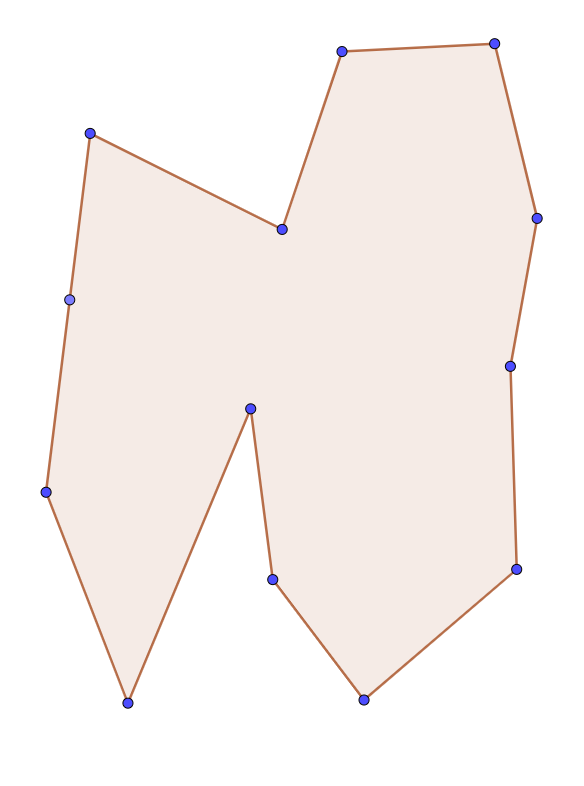
\includegraphics[width=\linewidth]{Images/intersection_polygon.png}
  \caption{A polygon that could be dissected}
  \label{fig:intersectionExamplePolygon}
\endminipage\hfill
\minipage{0.48\textwidth}
  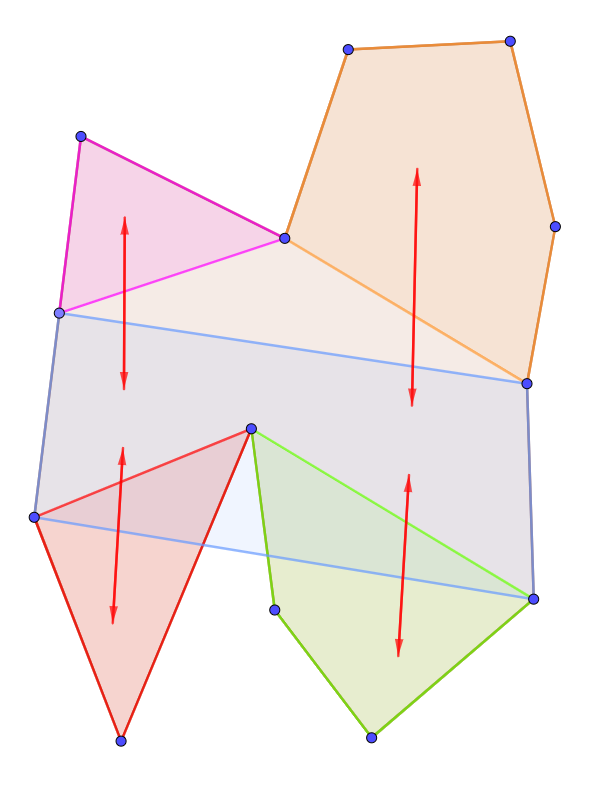
\includegraphics[width=\linewidth]{Images/intersection_yMonotoneSections.png}
  \caption{y-monotone sections of a polygon}
  \label{fig:intersectionPolygonSections}
\endminipage
\end{figure}

\begin{figure}[H]
\minipage{0.2\textwidth}
  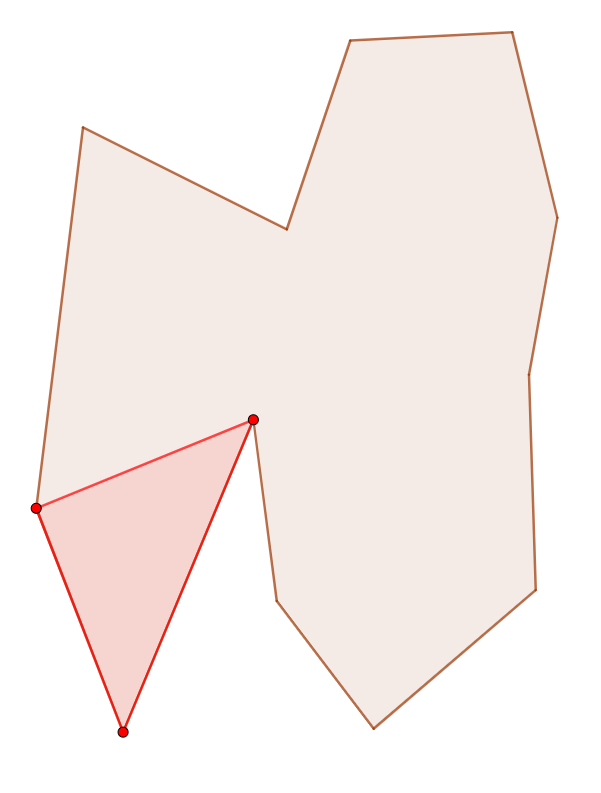
\includegraphics[width=\linewidth]{Images/intersection_yMonotoneSection1.png}
  \caption{}
  \label{fig:intersectionPolygonSection1}
\endminipage\hfill
\minipage{0.2\textwidth}
  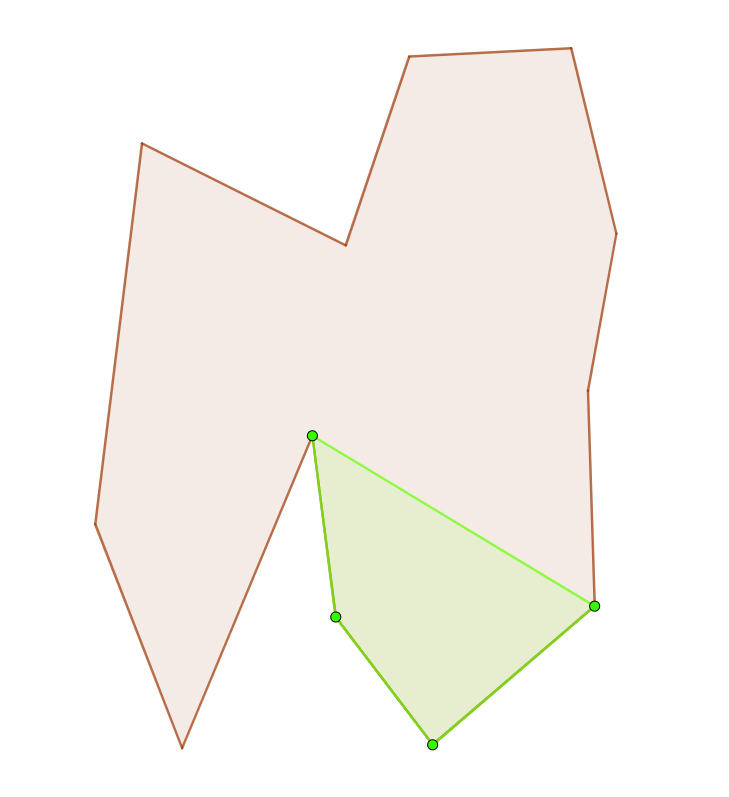
\includegraphics[width=\linewidth]{Images/intersection_yMonotoneSection2.png}
  \caption{}
  \label{fig:intersectionPolygonSection2}
\endminipage\hfill
\minipage{0.2\textwidth}
  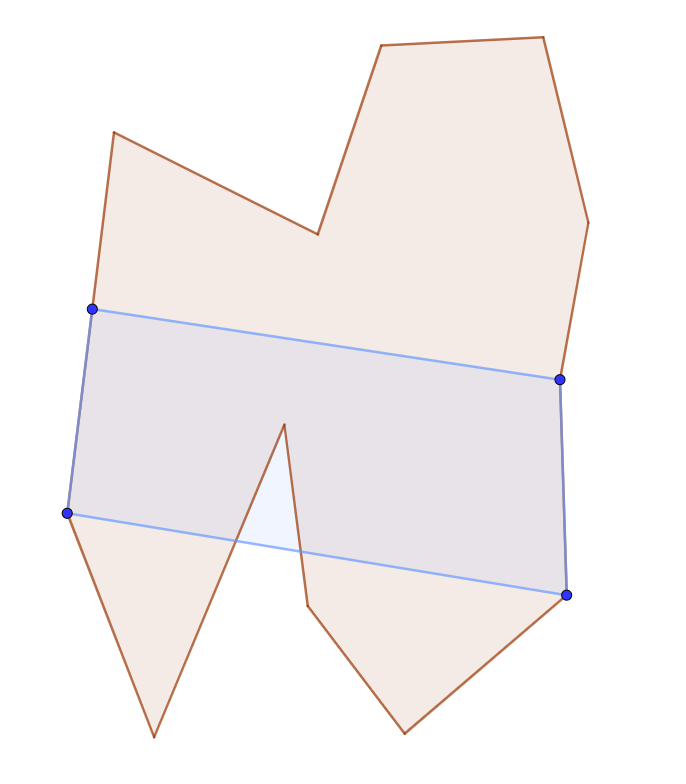
\includegraphics[width=\linewidth]{Images/intersection_yMonotoneSection3.png}
  \caption{}
  \label{fig:intersectionPolygonSection3}
\endminipage\hfill
\minipage{0.2\textwidth}
  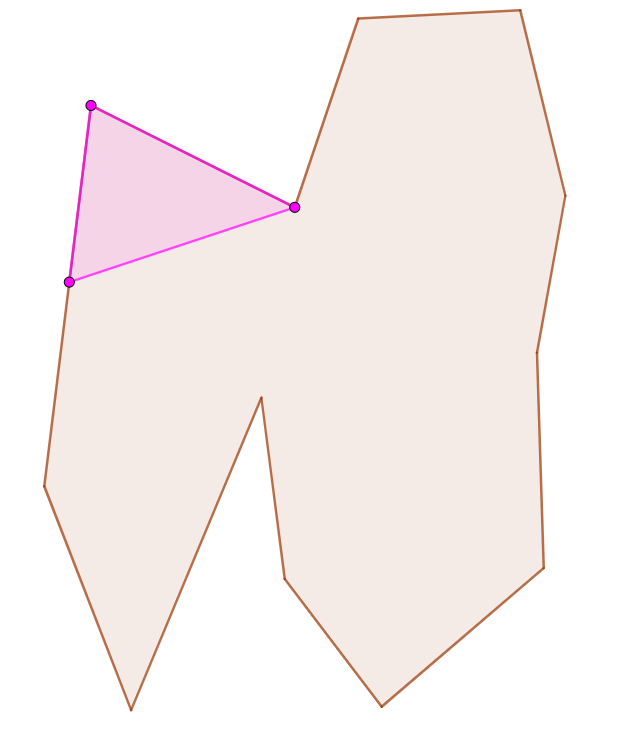
\includegraphics[width=\linewidth]{Images/intersection_yMonotoneSection4.png}
  \caption{}
  \label{fig:intersectionPolygonSection4}
\endminipage\hfill
\minipage{0.2\textwidth}
  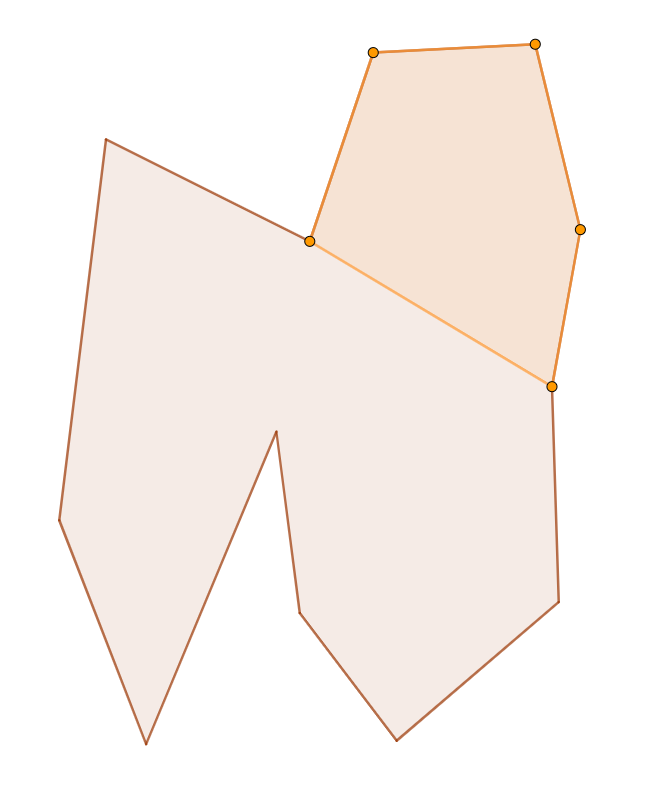
\includegraphics[width=\linewidth]{Images/intersection_yMonotoneSection5.png}
  \caption{}
  \label{fig:intersectionPolygonSection5}
\endminipage
\end{figure}

There are 7 different event types that of relevance when progressing the scanline. 6 of these can be calculated ahead of time for each input polygon individually, but the last one - intersection events - will be calculated at scantime. Below is a list of all event types and their colors withing Figure \ref{fig:intersectionEventTypes}. 
\begin{itemize}
    \item Interval start (light-green)
    \item Interval end (light-red)
    \item Interval split (dark-green)
    \item Interval merge (dark-red)
    \item Interval left wall replacement (light-blue)
    \item Interval right wall replacement (dark-blue)
    \item Interval boundaries intersection
\end{itemize}
The first 6 event types can be identified by walking the boundaries of the simple polygon and analyzing the relative positions of 3 consecutive points at a time to determine the even type corresponding to the middle of the three points.
Here an important edge case shows up, because determining the event types when dealing with horizontal lines is not very straight forward. We however managed to simplify this situation by imagining a symbolic left-rotation of the whole polygon that is small enough to not mess with the y-order of points (apart from points with the same y-value) in a similar fashion as was done in the vertical decomposition construction algorithm. An example of this is illustrated in Figures \ref{fig:intersectionHorizontalLines} and \ref{fig:intersectionHorizontalLinesRotated}. We also have to mirror this symbolic rotation in our event queue by having a lexicographical ordering which first sorts the events in increasing y-value followed by increasing x-value. 

\begin{figure}[H]
  \centering
  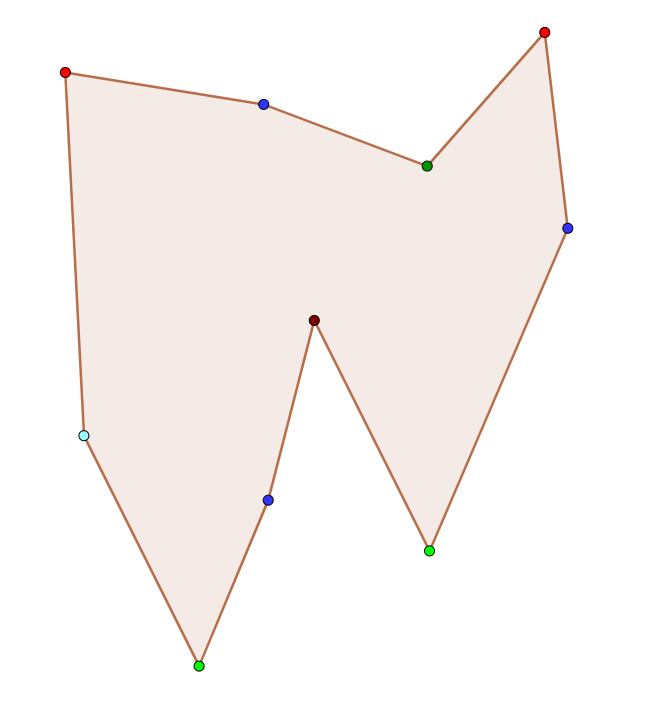
\includegraphics[width=0.5\linewidth]{Images/intersection_eventAssignment.png}
  \caption{The polygon event types}
  \label{fig:intersectionEventTypes}
\end{figure}
\begin{figure}[H]
\minipage{0.48\textwidth}
  \centering
  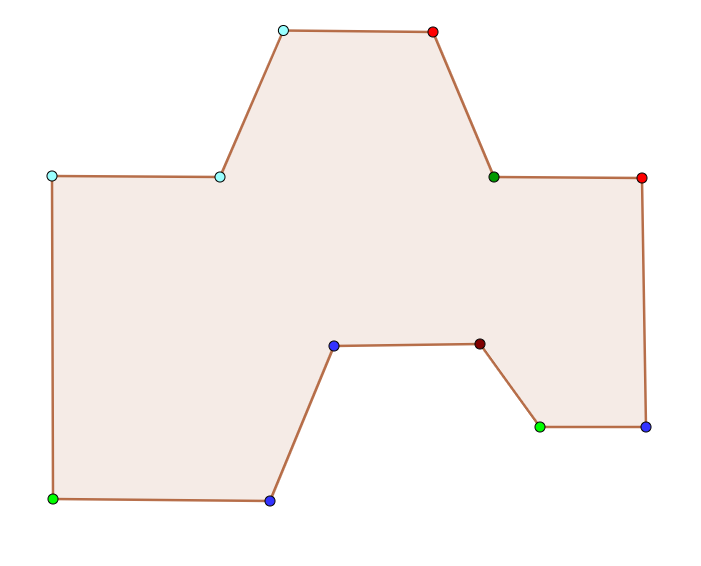
\includegraphics[height=5cm]{Images/intersection_eventAssignmentEdgeCase.png}
  \caption{Horizontal lines edge case}
  \label{fig:intersectionHorizontalLines}
\endminipage\hfill
\minipage{0.48\textwidth}
  \centering
  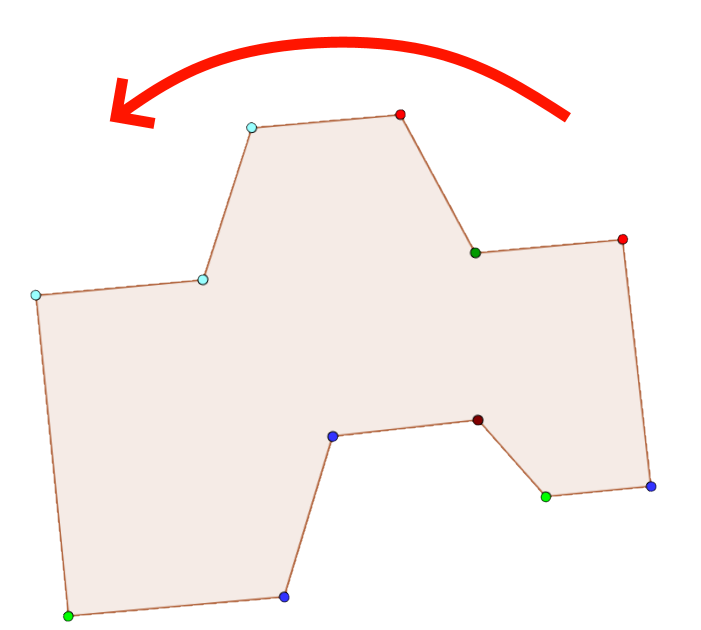
\includegraphics[height=5cm]{Images/intersection_eventAssignmentEdgeCaseRotated.png}
  \caption{Symbolic left rotation edge case fix}
  \label{fig:intersectionHorizontalLinesRotated}
\endminipage
\end{figure}

As stated before, the algorithm computes the intersections at runtime. Whenever a new interval is added to the scanline (or the boundary of an interval is altered) the interval will check whether its boundaries will intersect in the future. If they do intersect in the future, this intersection is added to the event queue. When an interval is removed from the scanline and its boundaries were going to intersect in the future, this intersection event is removed from the event queue. This can for instance happen if another line happened to intersect the boundary of an interval before the interval's boundaries intersected. 

Intersection events are handled completely separately from the other 6 event types. Moreover one has to be careful and consider that multiple events can take place in the same point. In this scenario where general position is not assumed the lexicographical event ordering has to be extended to prioritise intersection events over the other event types, the reason for which will become apparent later. Whenever an intersection event occurs interval $x$ whose boundaries intersected is retrieved, as well as interval $l$ that is to the left of $x$ and interval $r$ that is to the right of $x$. Now $x$'s boundaries are replaced together with the shared boundaries with $l$ and $r$ by new boundaries that stop at the intersection point. In Figure \ref{fig:intersectionIntersection} an intersection event is shown and the state after replacing the boundaries is highlighted in Figure \ref{fig:intersectionIntersectionOldBoundary}. Next a simple trick is used to offload all the other relevant logic to the normal event handling code. A new start event is created at the intersection point. This event stores the continuation of the left and right boundaries that we cut in two. Handling this even will take care of removing the stopped interval, updating its shape, updating $l$ and $r$'s shapes, and creating the new interval that was started. The creation of this even is illustrated in Figure \ref{fig:intersectionIntersectionNewStartEvent}

\begin{figure}[H]
\minipage{0.3\textwidth}
  \centering
  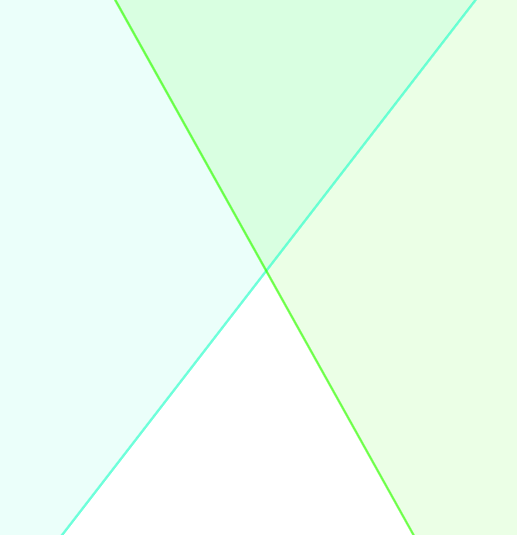
\includegraphics[height=5cm]{Images/intersection_intersect.png}
  \caption{An intersection situation}
  \label{fig:intersectionIntersection}
\endminipage\hfill
\minipage{0.3\textwidth}
  \centering
  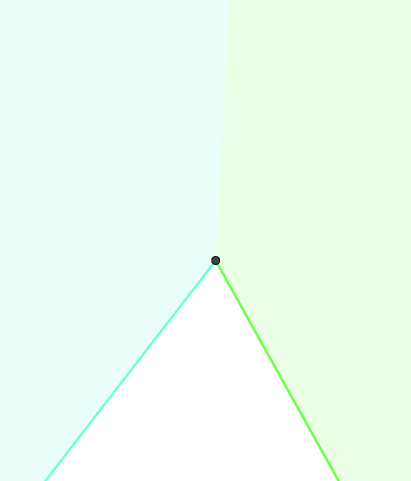
\includegraphics[height=5cm]{Images/intersection_intersectOldBoundaryCut.png}
  \caption{Intersection boundary replacement}
  \label{fig:intersectionIntersectionOldBoundary}
\endminipage\hfill
\minipage{0.3\textwidth}
  \centering
  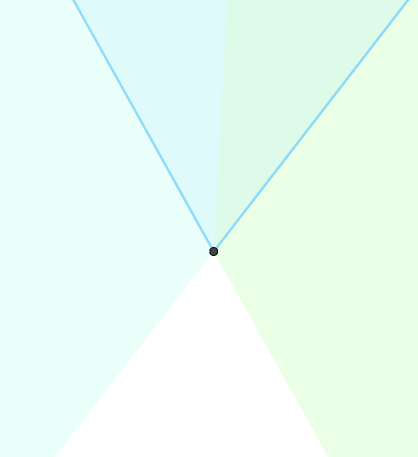
\includegraphics[height=5cm]{Images/intersection_intersectNewStartEvent.png}
  \caption{Intersection fake start event}
  \label{fig:intersectionIntersectionNewStartEvent}
\endminipage
\end{figure}

Handling all other 6 events is quite tricky at first glance, especially when considering multiple of these events can happen at the same point once again. They can however be generalized to simplify everything quite a bit: all that's important at a given point is knowing what new segments have started. So we will collect all non-intersection-events that start at the same point and handle them simultaneously. First off the scanline is queried for all intervals that contain the event point. Next we obtain all new boundaries (segments) of the events that occurred and sort them from left to right. Now using this data a couple of useful observations can be made: \begin{itemize}
    \item If there is more than 1 new boundary, new intervals should be created. More precisely, given $x$ new segments, there will be $x-1$ new intervals. This is illustrated in Figure \ref{fig:intersectionNewIntervals}.
    \item If there are more than 2 intervals that the event point lied in, there are intervals ending at this point. More precisely, given $n$ intervals containing the event point, there will be $n-2$ intervals that end. This is illustrated in Figure \ref{fig:intersectionOldIntervals}.
\end{itemize}

\begin{figure}[H]
\minipage{0.48\textwidth}
  \centering
  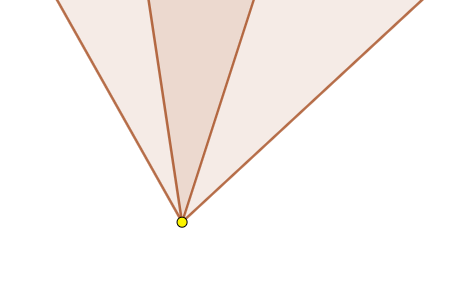
\includegraphics[height=5cm]{Images/intersection_newIntervals.png}
  \caption{Newly formed intervals}
  \label{fig:intersectionNewIntervals}
\endminipage\hfill
\minipage{0.48\textwidth}
  \centering
  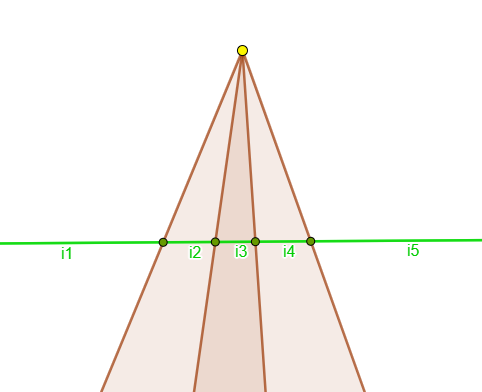
\includegraphics[height=5cm]{Images/intersection_oldIntervals.png}
  \caption{Old ended intervals (scanline moved down for clarity)}
  \label{fig:intersectionOldIntervals}
\endminipage
\end{figure}

This information can be exploited in the algorithm. One can quite easily cross the new boundaries from left to right and create the new intervals to add to the scanline. While crossing these boundaries the list of source polygons that are part of the interval can be tracked. Every segment of the event will store whether it was a left or right wall of a polygon, as well as the polygon itself. Thus when crossing a boundary one can add or remove the polygon from a list of sources, depending on whether it was a left or right wall.

Similarly all internal intervals (all intervals but the first and last) can be iterated over to remove them from the scanline, as well as add the event point to the shape's left and right walls.
Having taken care of these stopped and started intervals, only handling the outermost intervals remains. 3 different cases can be recognized here as illustrated in Figures \ref{fig:intersectionIntervalCase1} to \ref{fig:intersecionIntervalCase3}. Here the black triangles represent an unknown number of old/new boundaries, but there is at least 1 boundary such that the left and right parts of this triangle are separated. Each of these cases can be handled independently and are rather straight forward to handle. Case 1 and 3 will require new intervals to be created (with new y-monotone shapes), and case 2 only requires shapes and boundaries to be appropriately updated. Special care should be taken to properly link the new y-monotone sections with each other. Additionally all of these cases will check for new possible intersections. 

\begin{figure}[H]
\minipage{0.3\textwidth}
  \centering
  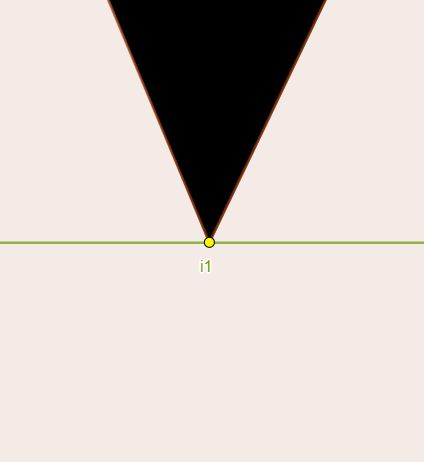
\includegraphics[height=5cm]{Images/intersection_case1.png}
  \caption{Shape linking case 1}
  \label{fig:intersectionIntervalCase1}
\endminipage\hfill
\minipage{0.3\textwidth}
  \centering
  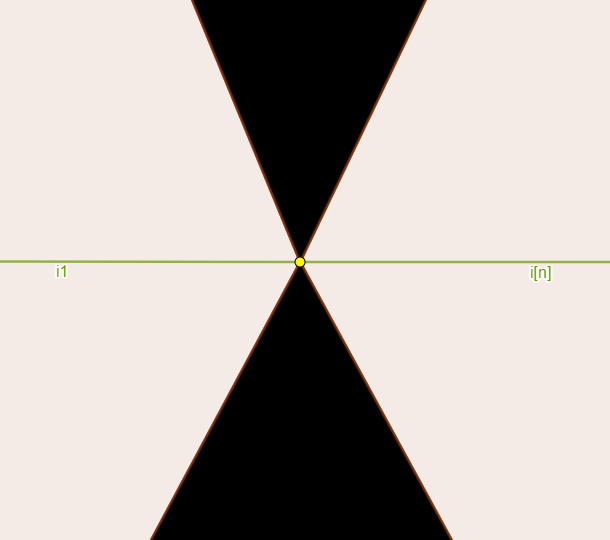
\includegraphics[height=5cm]{Images/intersection_case2.png}
  \caption{Shape linking case 2}
  \label{fig:intersecionIntervalCase2}
\endminipage\hfill
\minipage{0.3\textwidth}
  \centering
  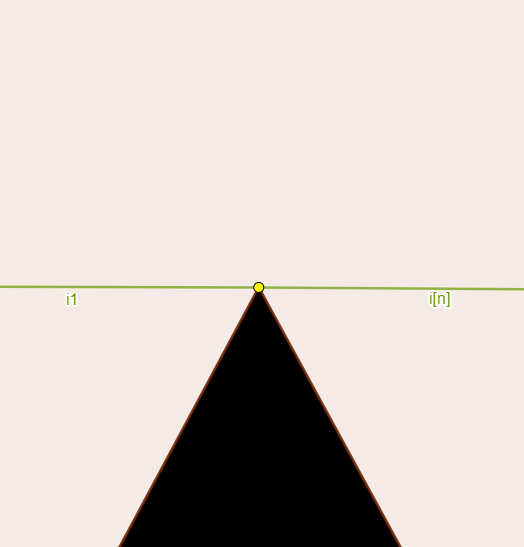
\includegraphics[height=5cm]{Images/intersection_case3.png}
  \caption{Shape linking case 3}
  \label{fig:intersecionIntervalCase3}
\endminipage
\end{figure}

This discussed approach still misses out on one significant edge case, but this is fortunately easy to handle: an event point may lie on a segment as illustrated in Figure \ref{fig:eventPointOnSegment}. This means that no pure intersection occurs, thus it would not be observed. When all intervals with the event point are retrieved this includes intervals with this segment as its boundary. Now one can easily iterate over all found intervals and if the event point lies on the boundary $b$ without being its endpoint, a new segment $s$ can be created starting at the event point and ending at the endpoint of $b$. These created segment are then added to the list of new boundaries starting at this event point. This ensures that the lines going through the point are properly considered in the rest of the calculation. This also handles the situation of multiple intersections occurring in the same point. If it were not for rounding errors this approach could take care of all intersection events, such that those would not have to be handled separately. It however is very plausible and not unlikely that a calculated intersection point does not lie exactly on both segments, which would make this approach fail in practice. But it is known that for a set of closed polygons that partially overlap either the segments will cross somewhere or a point will lie on a segment. Therefore the combination of the intersection approach and point on the segment approach will take care of all situations. 
\begin{figure}[H]
    \centering
    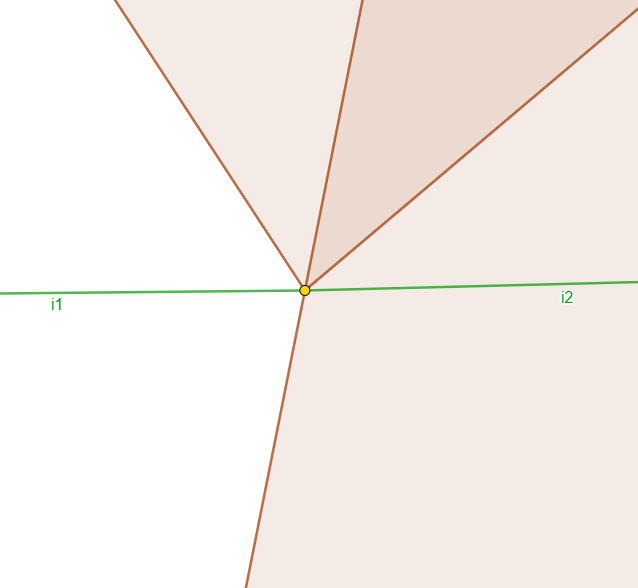
\includegraphics[width=10cm]{Images/intersection_pointOnSegment.png}
    \caption{Point lies on segment, but does not cross it}
    \label{fig:intersectionScanline}
\end{figure}

Now that events are handled in batches of the same point, this nuanced view of 7 different event types is excessive. Therefore in practice when the first 6 event types are identified, one can simply encode them within the 3 generalized virtual event types that the scanline later deals with:
\begin{itemize}
    \item Segment (start (2 instances), left wall, right wall, split)
    \item End (stop, merge)
    \item Intersection
\end{itemize}

\end{document}